\chapter{Electromagnetism}
\begin{center}
    \includegraphics[width=0.8\textwidth]{../images/Bar-Magnet/Bar-Magnet.pdf}
    \captionsetup{type=figure}
    \caption[figure]{\ref{Magnetic field produced by a bar magnet} Magnetic field produced by a bar magnet.}
\end{center}
\begin{itemize}
    \item A \emph{magnetic field} is a \emph{region of space} where a magnetic pole, moving charged particle or current-carrying conductor will \emph{experience a magnetic force}.
    \item Normally, a magnetic field points from north-to-south. However, \emph{inside} a magnet, the magnetic field points south-to-north. 
    \item A compass points in the same direction as the \(B\)-field.
    \begin{figure}[H]
        \centering
        \includegraphics[width=0.3\textwidth]{../images/compass.jpg}
        \caption{\ref{Me} Compass points in the same direction as the \(B\)-field}
        \label{fig:compass}
    \end{figure}
    \item \emph{Magnetic flux density} is defined as the \emph{force per unit current per unit length} acting on an \emph{infinitely long current-carrying conductor} placed \emph{perpendicularly} to the magnetic field.
    \item Dots and crosses as indicators of direction:
    \begin{center}
        \begin{tabular}{|Sc|Sc|}
            \hline
            \Large \(\bigotimes\) & Into the page\\
            \hline
            \Large \(\bigodot\) & Out of the page\\
            \hline
        \end{tabular}
    \end{center}
    \newpage
    \item Left and right hand rules:
    \begin{center}
        \includegraphics[width=0.5\textwidth]{../images/Left-Right-Hand-Rules/Left-hand-rule.png}
        \hspace{2cm}
        \includegraphics[width=0.28\textwidth]{../images/Left-Right-Hand-Rules/Right-hand-rule.pdf}
        \captionsetup{type=figure}
        \caption[figure]{\ref{Left and right hand rules} Left and right hand rules.}
    \end{center}
    \begin{example}{}{}
        Mark with a letter \(X\) the position where the resultant magnetic flux density is zero. Explain your reasoning \hspace*{\fill} [2]
        \begin{itemize}
            \item (Explain) To obtain zero magnetic flux density, the direction of the magnetic flux density due to current must be opposite that of the Earth. 
            \item (Direction) Using the right hand grip rule, this is to the east of the wire.
            \item (Distance) To have the same magnitude as the Earth's magnetic flux density, the position should be \rule{1cm}{0.01mm} (e.g. nearer than 19cm).
        \end{itemize} 
    \end{example}
    \item At any point some perpendicular distance \(d\) from the center of an \emph{infinitely long straight} current-carrying conductor, the magnitude of the magnetic flux is given by
    \[B=\frac{\mu_0I}{2\pi d}.\]
    Here, \(\mu_0=4\pi\cdot 10^{-7}\) is the permeability of free space.
    \begin{center}
        \includegraphics[width=0.5\textwidth]{../images/Current-Carrying-Wire/Current-Carrying-Wire.pdf}
        \captionsetup{type=figure}
        \caption[figure]{\ref{Current in a wire} Current in a wire.}
    \end{center}
    \item At the center of a flat circular coil with \(N\) turns, radius \(r\), and current \(I\) flowing through it, the magnitude of the magnetic flux density is given by 
    \[B=\frac{\mu_0NI}{2r}.\]
    \begin{center}
        \includegraphics[width=0.5\textwidth]{../images/Flat-Circular-Coil/Flat-Circular-Coil.pdf}        \captionsetup{type=figure}
        \caption[figure]{\ref{Flat circular coil} Current in a flat circular coil.}
    \end{center}
    \item Suppose we have an ideal (having infinite length) solenoid of \(n=N/L\) number of turns per unit length, which has a current \(I\) flowing through it. Then, the magnitude of the uniform magnetic flux density at its center is given by 
    \[B=\mu_0nI.\]
    \begin{center}
        \includegraphics[width=0.9\textwidth]{../images/Solenoid.pdf}
        \captionsetup{type=figure}
        \caption[figure]{\ref{Solenoid} Current in a solenoid and the magnetic field produced.}
    \end{center}
    \item A set of coils can be considered to be a solenoid when the radius of said coils is negligible compared to their length. 
    \item The addition of a ferrous core, of permeability \(\mu\), into a solenoid increases the magnetic flux density there, which is given by 
    \[B=\mu nI.\]
    \item Say we have a straight current-carrying conductor of length \(l\) with current \(I_\perp\) flowing perpendicular to the magnetic field. Then for any point on that conductor that experiences a magnetic flux of density \(B\), 
    \[F_B=BI_\perp l.\]
    \newpage
    \item ~
    \begin{center}
        \begin{tabular}{|Sc|Sc|}
            \hline
            Direction of Current in Two Wires & Direction of Net Magnetic Force\\
            \hline
            Same & Attractive\\
            \hline
            Opposite & Repulsive\\
            \hline
        \end{tabular} 
        \includegraphics[scale=1.5,page=1]{../images/Two-Current-Carrying-Wires/Two-Current-Carrying-Wires.pdf}

        \includegraphics[scale=1.5,page=2]{../images/Two-Current-Carrying-Wires/Two-Current-Carrying-Wires.pdf}
        \captionsetup{type=figure}
        \caption[figure]{\ref{Two current carrying conductors} Current carrying conductors in parallel.}
    \end{center}
    \item A charge \(q\) moving at speed \(v_\perp\) perpendicular to the magnetic field, of flux density \(B\), experiences a magnetic force of magnitude
    \[F_B=qv_\perp B.\]
    \item Notice that the charged particle above travels in circular motion, with radius and period
    \[r=\frac{mv}{Bq}\qquad\text{and}\qquad T=\frac{2\pi m}{qB}.\]
    \item Velocity selector. Suppose we have a velocity selector with a uniform magnetic field, of flux density \(B\) out of (or into) the paper. Further assume there is an electric field of strength \(E\) rightwards (or leftwards) in the selector. This is illustrated in \hyperlink{Fig-15.7}{Fig 15.7}. Then, for a charged particle perpendicular to both fields to pass (undeflected) through the slits, \(F_E=F_B\). This simplifies to 
    \[v=\frac{E}{B}.\]
    \begin{center}
        \hypertarget{Fig-15.7}{}
        \begin{minipage}{0.9\textwidth}
            \centering
            \raisebox{-0.5\height}{\includegraphics[width=0.45\textwidth,page=1]{../images/Velocity-Selector/Velocity-Selector.pdf}}
            \hspace*{.2in}
            \raisebox{-0.5\height}{\includegraphics[width=0.5\textwidth,page=2]{../images/Velocity-Selector/Velocity-Selector.pdf}}
            \captionsetup{type=figure}
            \caption[figure]{\ref{Velocity selector} An illustration of a velocity selector.}
          \end{minipage}
    \end{center}
\end{itemize}
\newpage
Some nice images:
\begin{center}
    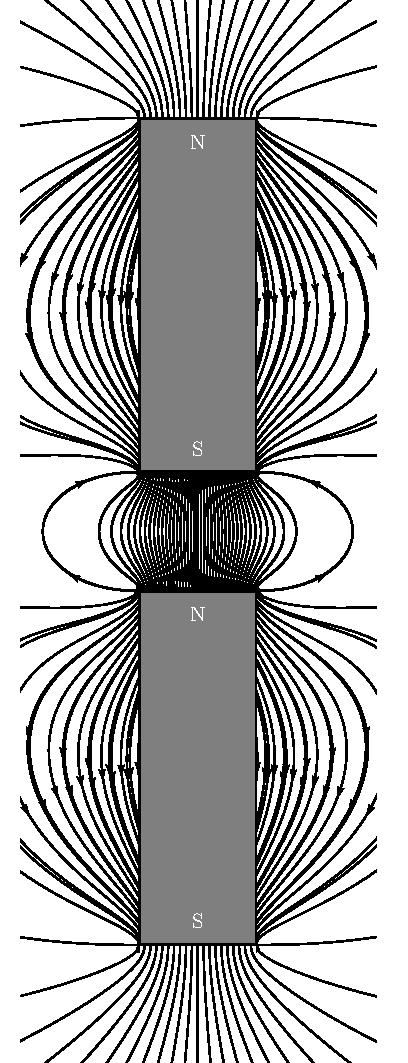
\includegraphics[angle=90,width=\textwidth]{../images/Bar-Magnet/Cropped/1.pdf}
    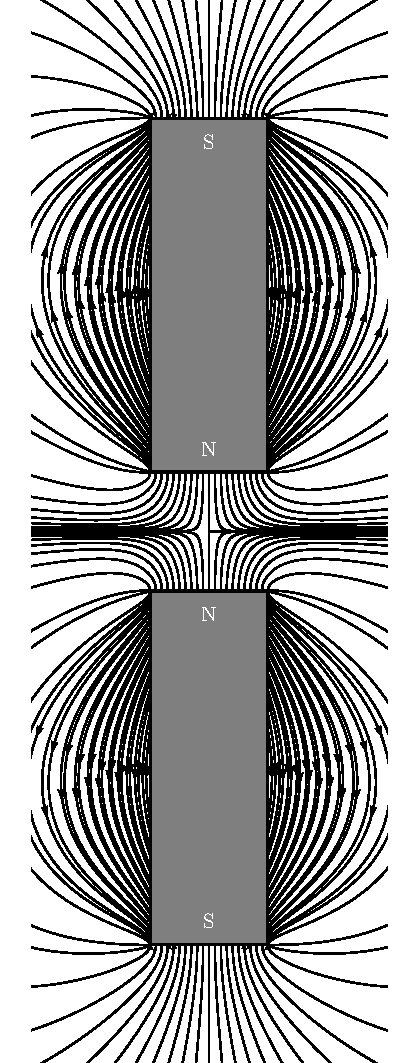
\includegraphics[angle=90,width=\textwidth]{../images/Bar-Magnet/Cropped/2.pdf}
    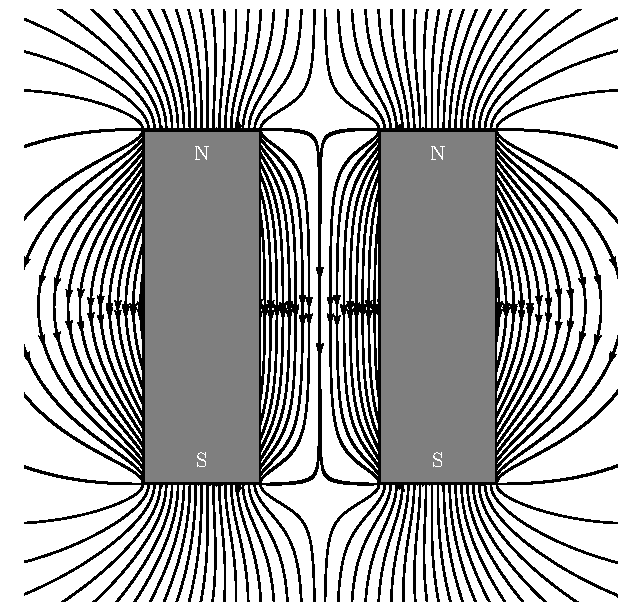
\includegraphics[width=0.49\textwidth]{../images/Bar-Magnet/Cropped/3.pdf}
    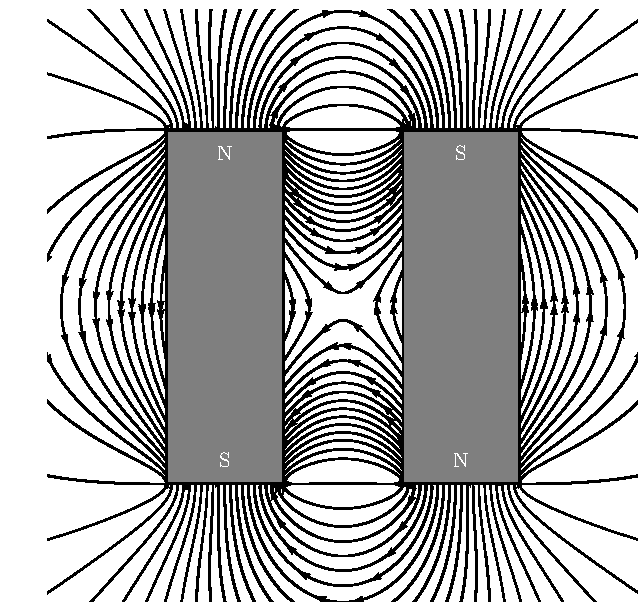
\includegraphics[width=0.49\textwidth]{../images/Bar-Magnet/Cropped/4.pdf}
    \captionsetup{type=figure}
    \caption[figure]{\ref{Magnetic field produced by a bar magnet} Magnetic fields produced by two bar magnets.}
\end{center}